\documentclass[11pt,a4paper]{article}

% ── Packages ──────────────────────────────────────────────────────────
\usepackage[utf8]{inputenc}
\usepackage[T1]{fontenc}
\usepackage{lmodern}
\usepackage[margin=2.5cm]{geometry}
\usepackage{graphicx}
\usepackage{hyperref}
\usepackage{xcolor}
\usepackage{listings}
\usepackage{booktabs}
\usepackage{longtable}
\usepackage{enumitem}
\usepackage{tikz}
\usetikzlibrary{arrows.meta, positioning, shapes.geometric, fit, calc}
\usepackage{amsmath}
\usepackage{fancyhdr}
\usepackage{tocloft}

% ── Colour Palette ────────────────────────────────────────────────────
\definecolor{codeblue}{HTML}{0060A8}
\definecolor{codered}{HTML}{FF3333}
\definecolor{codegray}{HTML}{5A5A5A}
\definecolor{codegreen}{HTML}{008040}
\definecolor{codebg}{HTML}{F5F5F5}
\definecolor{linkblue}{HTML}{1A5276}

% ── Hyperref Setup ────────────────────────────────────────────────────
\hypersetup{
  colorlinks=true,
  linkcolor=linkblue,
  citecolor=linkblue,
  urlcolor=linkblue
}

% ── Listings Setup ────────────────────────────────────────────────────
\lstset{
  basicstyle=\ttfamily\small,
  keywordstyle=\color{codeblue}\bfseries,
  commentstyle=\color{codegray}\itshape,
  stringstyle=\color{codegreen},
  backgroundcolor=\color{codebg},
  frame=single,
  framerule=0.4pt,
  rulecolor=\color{codered!80},
  breaklines=true,
  showstringspaces=false,
  tabsize=4,
  captionpos=b,
  xleftmargin=1em,
  framexleftmargin=0.5em
}

\lstdefinelanguage{CSV}{
  morecomment=[l]{\#},
  morestring=[b]",
}

% ── Headers / Footers ────────────────────────────────────────────────
\pagestyle{fancy}
\fancyhf{}
\fancyhead[L]{\small Komondor Developer Guide}
\fancyhead[R]{\small\thepage}
\renewcommand{\headrulewidth}{0.4pt}

% ── Title ─────────────────────────────────────────────────────────────
\title{%
  \vspace{-1cm}
  {\LARGE\bfseries Kom8ndor's Developer Guide}\\[6pt]
  {\large Last update: July 2026}
}
\author{Auto-generated from source analysis \& Manually edited by F. Wilhelmi}
\date{}

% ══════════════════════════════════════════════════════════════════════
\begin{document}
\maketitle
\tableofcontents
\newpage

% ======================================================================
\section{Introduction}
% ======================================================================

\texttt{Kom8ndor}\footnote{This is the name we gave to the Wi-Fi 8 extension of Komondor.} is a discrete-event IEEE 802.11bn-oriented network simulator written in C++98 on top of the CompC++/COST simulation framework.  It models the full MAC/PHY protocol and includes functionalities such as channel bonding, spatial reuse, beamforming, EDCA, and Multi-AP Coordination (MAPC). It also integrates Machine Learning (ML) functionalities through a Reinforcement Learning (RL) subsystem for online parameter tuning and a socket-based integration for Python.

The codebase is approximately 112\,000 lines of code spread across roughly 30 header files and 5 \texttt{.cc} translation units.  Almost all logic lives in \texttt{.h} files because the COST preprocessor inlines component method bodies.

\subsection{Scope of This Guide}

This guide is intended to introduce the internal behavior of \texttt{Kom8ndor} to any interested researcher/practitioner who would like to extend/modify the source code. In particular, this document provides:
\begin{itemize}[nosep]
  \item A map of the directory structure and file responsibilities.
  \item An explanation of the CompC++/COST execution model.
  \item A walk-through of the node finite-state machine (FSM).
  \item Descriptions of every major subsystem: backoff, channel access, power/SINR, beamforming, MAPC, NPCA/DSO, EDCA, and ML.
  \item Input/output CSV formats and how to create new scenarios.
  \item Build instructions.
\end{itemize}

% ======================================================================
\section{Repository Layout}
\label{sec:layout}
% ======================================================================

\begin{lstlisting}[language={},caption={Top-level directory tree.}]
Komondor/
  Apps/                  Post-processing & plotting utilities
  Code/
    COST/                CompC++ simulation framework (Linux ELF)
    input/               Input scenarios (CSV files)
    learning_modules/    ML/RL components
    main/                Main files & components and Makefile
    methods/             Implementation logic headers
      channel/           Power, SINR, beamforming
      frames/            Notifications, aggregation logic
      mac/               Backoff, channel access, NAV, losses
      mapc/              Multi-AP Coordination methods
      node/              Node FSM helpers, packet, timeout, backoff
      utils/             Input loader, output writer
      phy/               Modulations, beamforming, channel bonding
    output/              Placeholder for simulation outputs
    scripts_multiple_executions         Examples of scripts to run multiple scenarios
    structures/          Data structures (NodeParameters, Wlan...)
    config_models        File with global models
    list_of_macros       File with macros
    validate             File that runs regression tests
  Documentation/         Docs & tutorials
\end{lstlisting}

\subsection{Source Files at a Glance}

We next list every source file under \texttt{Code/} with its approximate role. More detailed descriptions of each block are provided throughout this document.

\subsubsection{Code/COST}

The COST folder is a third-party discrete-event simulation framework from Rensselaer Polytechnic Institute (authors: Gilbert Chen, Boleslaw Szymanski, Mark Lisee; circa 2003–2007). COST stands for Component-Oriented Simulation Toolkit, layered here with the SENSE (Simulator for wirElEss Network Simulation Experiments) library on top of it.

\subsubsection{Code/input}

Includes input CSV files to define simulation scenarios. It contains two baseline folders:
\begin{itemize}
    \item \texttt{Code/input/examples}: Contains examples for different features (bandwidth adaptation, basic example, DSO and NPCA, EDCA, external ML model...).
    \item \texttt{Code/input/validation}: Contains the files used by the regression tests (see \texttt{validate.sh}).
\end{itemize}

\subsubsection{Code/learning\_modules/}

\begin{itemize}
    \item \texttt{action\_space.h}: Action encoding/decoding.
    \item \texttt{agent\_methods.h}: Agent helper functions, including performance-metric reset and data-validity checks.
    \item \texttt{external\_model\_client.h}: Unix-socket client for external Python ML servers.
    \item \texttt{learning\_algorithm.h}: Algorithm dispatcher (MAB, RTOT\footnote{Ropitault, T. (2018, January). Evaluation of RTOT algorithm: A first implementation of OBSS\_PD-based SR method for IEEE 802.11 ax. In 2018 15th IEEE Annual Consumer Communications \& Networking Conference (CCNC) (pp. 1-7). IEEE.}, external model).
    \item \texttt{ml\_model.h}: Legacy ML model (used by \texttt{CentralController}).
    \item \texttt{pre\_processor.h}: Thin coordinator over reward/action/algorithm.
    \item \texttt{reward\_function.h}: Reward computation (throughput-based, fairness...).
    \item \textit{Code/learning\_modules/network\_optimization\_methods/}
    \begin{itemize}
        \item \texttt{centralized\_action\_banning.h}: Used to ban low-performing actions across all agents under central-controller coordination, with rollback support.
        \item \texttt{multi\_armed\_bandits.h}: Implements $\varepsilon$-greedy, UCB1, and Thompson Sampling strategies.\footnote{Lattimore, T., \& Szepesvári, C. (2020). Bandit algorithms. Cambridge University Press.}
        \item \texttt{rtot\_algorithm.h}: \texttt{RtotAlgorithm} class implementing the Recommended TX Output Threshold algorithm for adaptive OBSS-PD tuning.
    \end{itemize}
    \item \textit{Code/learning\_modules/python\_servers/}
    \begin{itemize}
        \item \texttt{ml\_server\_passthrough.py}: Smoke-test server that echoes the received arm index back unchanged; useful for verifying socket connectivity.
        \item \texttt{ml\_server\_random.py}: Baseline server that selects a random arm each step; reads the number of arms from the feature vector sent by the simulation.
        \item \texttt{ml\_server\_pytorch.py}: PyTorch inference / online-RL server; loads a TorchScript model and returns the action predicted by a forward pass.
        %\item \texttt{ml\_server\_channel\_access.py}: RL server for ML-learned channel access; replaces the DCF backoff with a learned policy queried at per-TXOP granularity.
        %\item \texttt{generate\_scenario.py}: Scenario generator for ML channel access training and testing; produces Komondor node CSVs with controlled or randomised parameters, and can generate matched DCF-baseline topologies for fair comparison.
    \end{itemize}
\end{itemize}


\subsubsection{Code/main}

\begin{itemize}
    \item \texttt{agent.h}: ML agent component, with interactions with nodes, other agents, and the central controller.
    \item \texttt{build\_local}: Script that builds the code from the pre-compiled cxx COST engine (platform-dependent). The Makefile (added later and the preferred way to build now) does the same steps but also adds dependency tracking (it watches all .cc and .h files and rebuilds only when something has changed).
    \item \texttt{central\_controller.h}: Centralized multi-WLAN coordination that handles agents associated with it.
    \item \texttt{komondor\_main.cc}: Entry point, including CLI parsing, component wiring, and simulation loop.
    \item \texttt{Makefile}: Defines build rules to compile the source code (\texttt{g++ -std=c++98}).
    \item \texttt{node.h}: Monolithic node component, including all the interactions that occur during the simulation.
    \item \texttt{traffic\_generator.h}: Module that generates traffic for nodes. Includes traffic models such as \textit{full-buffer}, \textit{Poisson}, and \textit{deterministic}.
\end{itemize}



\subsubsection{Code/methods}

\begin{itemize}
    \item \textit{Code/methods/frames/}
    \begin{itemize}
        \item \texttt{notification\_methods.h}: Builds the \texttt{TxInfo} struct embedded in every \texttt{Notification} (\texttt{GenerateTxInfo}); called by \texttt{GenerateNotification()} inside \texttt{node.h}.
        \item \texttt{packet\_aggregation\_methods.h}: Computes the maximum A-MPDU aggregation level (\texttt{FindMaximumPacketsAggregated}) given the current MCS, channel bandwidth, and remaining TXOP budget.
    \end{itemize}
    %
    \item \textit{Code/methods/mac/}
    \begin{itemize}
        \item \textit{Code/methods/mac/channel\_access/}
        \begin{itemize}
            \item \texttt{backoff\_methods.h}: Binary exponential backoff and EDCA backoff dispatcher; entry point for all backoff-type computations.
            \item \texttt{channel\_access\_methods.h}: Channel access policy abstraction (\texttt{ChannelAccessPolicy} strategy struct); registers the CCA-check and channel-bonding selection logic used when a backoff expires.
            \item \texttt{dcf\_methods.h}: DCF random-slot backoff (uniform draw in $[0, \text{CW})$).
            \item \texttt{deterministic\_backoff\_methods.h}: Deterministic backoff schedule (Qualcomm variant\footnote{Kosek-Szott, K., Szott, S., Valvo, A. L., \& Tinnirello, I. (2022, October). Db-lbt: Deterministic backoff with listen before talk for wi-fi/nr-u coexistence in shared bands. In 2022 30th International Symposium on Modeling, Analysis, and Simulation of Computer and Telecommunication Systems (MASCOTS) (pp. 168-175). IEEE.}).
            \item \texttt{eca\_methods.h}: Enhanced Channel Access (ECA) backoff variant.\footnote{Sanabria-Russo, L., Barcelo, J., Bellalta, B., \& Gringoli, F. (2016). A high efficiency MAC protocol for WLANs: Providing fairness in dense scenarios. IEEE/ACM Transactions on Networking, 25(1), 492-505.}
            \item \texttt{edca\_methods.h}: EDCA per-access-category binary exponential backoff with AIFSN computation.
            %\item \texttt{ml\_access\_methods.h}: ML-driven channel access; queries an external Python server via socket to obtain the next backoff value.
            \item \texttt{tokenized\_backoff\_methods.h}: Token-based channel access backoff.\footnote{Wilhelmi, F., Galati-Giordano, L., \& Fontanesi, G. (2025, March). “It's Your Turn”: A Novel Channel Contention Mechanism for Improving Wi-Fi's Reliability. In 2025 IEEE Wireless Communications and Networking Conference (WCNC) (pp. 1-6). IEEE.}
        \end{itemize}
        \item \texttt{nack\_methods.h}: Generates and processes logical NACKs for collision and decoding-failure events (\texttt{GenerateLogicalNack}, \texttt{ProcessNack}).
        \item \texttt{nav\_methods.h}: Computes NAV duration values (\texttt{ComputeNavTime}) for RTS, CTS, DATA, ACK, ICF, and TF frames, so that neighbouring nodes set their virtual carrier-sense timer correctly.
        \item \texttt{packet\_loss\_methods.h}: Packet loss decision logic (\texttt{HandlePacketLoss}, \texttt{CanDecodePacket}, \texttt{IsPacketLost}); applies the SINR threshold, capture-effect model, and constant PER override.
        \item \texttt{spatial\_reuse\_methods.h}: BSS-colour-based SR helpers: packet-origin classification (\texttt{CheckPacketOrigin}), OBSS-PD sensitivity selection (\texttt{GetSensitivitySpatialReuse}), SR opportunity identification (\texttt{IdentifySpatialReuseOpportunity}), and TX-power restriction (\texttt{ApplyTxPowerRestriction}).
    \end{itemize}
    %
    \item \textit{Code/methods/mapc/}
    \begin{itemize}
        \item \texttt{mapc\_methods.h}: MAPC coordinator helpers for peer-AP selection logic (\texttt{selectMapcPeer}, used for round-robin TXOP allocation) and Co-SR transmit-power calculation (used in the coordinated power adaptation path).
    \end{itemize}
    %
    \item \textit{Code/methods/node/}
    \begin{itemize}
        \item \texttt{node\_backoff\_methods.h}: DIFS/EIFS handling, EndBackoff dispatch.
        \item \texttt{node\_fsm\_methods.h}: Setup, Start, Stop, InitializeVariables, RestartNode.
        \item \texttt{node\_packet\_methods.h}: PrepareNewTransmission, GenerateNotification, MyTxFinished.
        \item \texttt{node\_timeout\_methods.h}: ACK/CTS/DATA/NPCA timeout handlers.
    \end{itemize}
    %
    \item \textit{Code/methods/phy/}
    \begin{itemize}
        \item \texttt{beamforming\_methods.h}: ULA beam-weight computation for standalone and coordinated beamforming, including projection null-steerer (Gram--Schmidt, \texttt{ComputeBeamWeights}) and Zero-Forcing precoding (\texttt{ComputeZFBeamWeights}), plus \texttt{ComputeRxBeamGain} to apply the resulting gain at the receiver.
        \item \texttt{channel\_bonding\_methods.h}: Channel-bonding selection logic for IEEE 802.11ax and beyond. The main entry point \texttt{GetTxChannelsByChannelBondingCCA11ax} evaluates per-subchannel CCA thresholds (primary at $-82$\,dBm, secondaries at $-72$\,dBm) and returns the widest feasible contiguous power-of-two bandwidth, up to 320\,MHz, for all supported bonding models.
        \item \texttt{frame\_duration\_methods.h}: Frame-duration calculations for all IEEE 802.11ax MAC frame types: \texttt{ComputeTxTime} (generic bits/rate formula), \texttt{ComputeRtsTxTime80211ax}, \texttt{ComputeCtsTxTime80211ax}, and \texttt{ComputeDataTxTime80211ax} (accounts for A-MPDU aggregation level and packet length). Also defines the \texttt{Exponential} random-variate helper used for stochastic transmission-time modelling.
        \item \texttt{mcs\_methods.h}: MCS selection and link-quality helpers. \texttt{SelectMCSResponse} maps a received power level to the highest feasible MCS index using RSSI thresholds that scale with channel width ($+3$\,dB per doubling of bandwidth). \texttt{ComputeEbToNoise} converts SINR, bit rate, bandwidth, and modulation type into an $E_b/N_0$ value for PER evaluation.
        \item \texttt{power\_channel\_methods.h}: Path-loss computation, per-node received-power tracking (\texttt{UpdatePowerSensedPerNode}, with beamforming gain applied to DATA frames only), SINR calculation, and the \texttt{ConvertPower} utility for unit conversions between pW, mW, and dBm.
    \end{itemize}
    %
    \item \textit{Code/methods/utils/}
    \begin{itemize}
        \item \textit{Code/methods/utils/input\_methods/}
        \begin{itemize}
            \item \texttt{input\_loader.h}: CSV parsing for all input files. Reads \texttt{config\_models} and performs a two-pass parse of the node CSV (first pass identifies WLANs, second pass instantiates nodes and STAs); further functions load MAPC group files and agent CSV files.
            \item \texttt{input\_validator.h}: Post-load sanity checks on the assembled node container (\texttt{ValidateInput}): verifies TX power and sensitivity are within admissible ranges, checks that channel assignments are consistent, and detects duplicate node IDs or positions.
        \end{itemize}
        \item \texttt{auxiliary\_methods.h}: General-purpose helpers used across the codebase: \texttt{ToString} (generic value-to-string conversion), array utilities (e.g., \texttt{PickRandomElementFromArray}), and numeric helpers (\texttt{RandomDouble}, \texttt{TruncateDouble}, \texttt{RoundToDigits}).
        \item \texttt{logging\_methods.h}: Low-level log-writing helpers shared by all components. Formats integer and floating-point arrays into the node log file or console.
        \item \texttt{output\_generation\_methods.h}: End-of-simulation statistics and formatted output. Aggregates per-node \texttt{Performance} objects into a \texttt{SimulationStats} summary and dispatches to one of several scenario-specific formatters (toy two-WLAN scenario, large node-density scenario, central-WLAN detailed counters, Bianchi multi-WLAN analysis, etc.) selected by the \texttt{simulation\_ix\_output\_script} field in \texttt{config\_models}.
        \item \texttt{print\_and\_write\_methods.h}: \texttt{Kom8ndor}-level diagnostic printers called at simulation start and end (e.g., \texttt{PrintSystemInfo}/\texttt{WriteSystemInfo}). These produce the human-readable header block visible at the top of every log file.
    \end{itemize}    
\end{itemize}

\subsubsection{Code/scripts\_multiple\_executions}

Contains three Bash helper scripts for running batches of simulations. All scripts trigger a \texttt{make} build before executing and append every result to a single output file. They are run from the \texttt{Code/scripts\_multiple\_executions/} directory on Linux, and their key parameters (input folder, number of seeds, agents file) can be overridden via environment variables without editing the scripts.

\begin{itemize}
    \item \texttt{multiple\_inputs\_script.sh}: Runs \texttt{komondor\_main} once per \texttt{input\_nodes*.csv} file found in a given input folder, using a fixed seed. Useful for running simulation campaigns.
    \item \texttt{multiple\_inputs\_script\_several\_seeds.sh}: Extends the above by repeating each scenario file across $N$ different random seeds (default 5), allowing statistical averaging of results.
    \item \texttt{multiple\_inputs\_script\_agents.sh}: Runs \texttt{komondor\_main} with a shared agents CSV file paired against every node file in a given folder. Intended for ML-agent experiments where the same learning configuration is evaluated across multiple topologies.
\end{itemize}

\subsubsection{Code/structures}

\begin{itemize}
    \item \texttt{action.h}: One discrete arm in the learning action space, storing the associated channel, CCA threshold, TX power, and maximum bandwidth, together with reward statistics and play counters tracked since the last controller request.
    \item \texttt{agent\_capabilities.h}: Advertises to the central controller which action dimensions (channel, power, sensitivity, bandwidth) a given agent is allowed to tune.
    \item \texttt{channel\_access\_state.h}: Groups the live backoff countdown, current contention-window stage and bounds, deterministic-backoff phase flag, and ECA/repeat-BO state that would otherwise be scattered as private variables in \texttt{node.h}.
    \item \texttt{controller\_report.h}: The shared state held by the central controller, including per-agent last configuration and performance snapshots, cluster membership arrays, and per-agent action-statistics matrices used for centralized action banning.
    \item \texttt{FIFO.h}: A simple packet queue wrapping an array of \texttt{Notification} objects, with methods to enqueue (\texttt{PutPacket}, \texttt{PutPacketFront}, \texttt{PutPacketIn}), dequeue (\texttt{DelFirstPacket}, \texttt{DeletePacketIn}), and inspect (\texttt{GetFirstPacket}, \texttt{GetPacketAt}, \texttt{QueueSize}).
    \item \texttt{logger.h}: A file pointer paired with a write-enable flag, passed into every method that produces per-node log output.
    \item \texttt{logical\_nack.h}: Carries the packet type, packet ID, source and destination node IDs, and loss-reason code exchanged when a transmission fails.
    \item \texttt{modulations.h}: Look-up tables for the MCS entries (modulation bits and coding rates), plus the helper \texttt{GetNumberSubcarriers()} that maps a channel count to the corresponding OFDM subcarrier count (20\,MHz through 320\,MHz).
    \item \texttt{node\_configuration.h}: The runtime tunable state of a node: primary channel, packet-detection threshold, TX power, maximum bandwidth, and spatial-reuse parameters. This is the type exchanged between nodes and their ML agents.
    \item \texttt{node\_parameters.h}: Static per-node configuration loaded once from the node CSV (identity, position, channel range, channel-bonding model, default TX power, CCA threshold, traffic model, protocol variant, etc.).
    \item \texttt{node\_statistics.h}: All runtime counters and measurements for a node, organized into categories: packet/frame counters, throughput/delay/utilization, backoff history, channel-idle tracking, NAV tracking, MAPC/TXOP-sharing statistics, rolling-window per-period stats, and dynamically allocated per-channel and per-STA arrays.
    \item \texttt{notification.h}: The message broadcast between nodes on every transmission event, carrying source/destination IDs, packet type, channel range, TX power, NAV time, MCS, beamforming parameters, MAPC allocation fields, spatial-reuse fields, and preamble-puncturing mask.
    \item \texttt{packet\_exchange\_sequence.h}: Defines the ordered list of MAC frame types for each supported exchange mode, with pre-built static instances: \texttt{IEEE\_802\_11\_NO\_RTS\_CTS}, \texttt{IEEE\_802\_11\_RTS\_CTS}, \texttt{IEEE\_802\_11\_COTDMA}, \texttt{IEEE\_802\_11\_COBF\_COSR}, \texttt{IEEE\_802\_11\_DSO}, and \texttt{IEEE\_802\_11\_NPCA}.
    \item \texttt{performance.h}: Per-measurement-window snapshot reported from a node to its agent: throughput, maximum-bound throughput, packets sent/lost/ACKed, RTS/CTS counters, delay statistics, channel utilization, per-WLAN RSSI list, and received-power array.
    \item \texttt{sim\_configuration.h}: Aggregates all CLI and \texttt{config\_models} inputs into a single object passed through the simulation: logging flags, simulation time and seed, feature-enable flags (agents, MAPC, beamforming, DSO, NPCA, ...), physical-layer model selections, and agent action-space definitions.
    \item \texttt{simulation\_stats.h}: Aggregated statistics accumulated across all nodes for the full simulation run, replacing former module-scope global variables.
    \item \texttt{spatial\_reuse\_state.h}: Groups the spatial-reuse runtime state (SR enable flag, TXOP-SR identification flag, current OBSS-PD threshold, TX-power restriction, Co-SR active flag, and related fields) that would otherwise be private variables in \texttt{node.h}.
    \item \texttt{wlan.h}: WLAN-level configuration: AP and STA node IDs, channel-bonding policy, MAPC group arrays (up to \texttt{MAX\_MAPC\_GROUPS\_PER\_WLAN}), beamforming parameters, DSO/NPCA enable flags, and EDCA per-AC parameters.
\end{itemize}


\subsubsection{Code/config\_models}

A plain-text key-value configuration file (no extension) read by the simulator at start-up to set global physical-layer and MAC model choices independently of any scenario CSV. The fields it controls are:

\begin{itemize}
    \item \texttt{adjacent\_channel\_model}: Selects the adjacent-channel interference model.
    \item \texttt{collisions\_model}: Selects how simultaneous-transmission collisions are resolved.
    \item \texttt{path\_loss\_model}: Selects the propagation model applied to all node pairs (e.g., free-space, Okumura--Hata urban, IEEE 802.11ax indoor).
    \item \texttt{simulation\_ix\_output\_script}: Integer index appended to batch-script output filenames for book-keeping.
\end{itemize}

\subsubsection{Code/list\_of\_macros.h}

The single header included by virtually every other file. It is the authoritative source of all named integer constants used across the simulator and is organized into the following groups:

\begin{itemize}
    \item \textbf{Boolean}: \texttt{TRUE}/\texttt{FALSE}.
    \item \textbf{Node FSM states}: core 802.11 states (\texttt{STATE\_SENSING}, \texttt{STATE\_TX\_DATA}, \texttt{STATE\_NAV}, etc.), MAPC coordination states (\texttt{STATE\_TX\_ICF}, \texttt{STATE\_RX\_ICR}, \texttt{STATE\_TX\_TF}, ...), DSO states (\texttt{STATE\_TX\_DSO\_ICF}, ...), and NPCA states (\texttt{STATE\_TX\_NPCA\_ICF}, ...).
    \item \textbf{Node types}: \texttt{NODE\_TYPE\_AP} / \texttt{NODE\_TYPE\_STA}.
    \item \textbf{Packet types}: \texttt{PACKET\_TYPE\_DATA}, \texttt{ACK}, \texttt{RTS}, \texttt{CTS}, \texttt{MCS\_REQUEST}, \texttt{MCS\_RESPONSE}, and all MAPC (\texttt{ICF}, \texttt{ICR}, \texttt{TF}, \texttt{MU\_RTS\_TXS}), DSO, and NPCA frame types.
    \item \textbf{Logical NACK reasons}: enumeration of collision and loss causes.
    \item \textbf{Path-loss models}: free-space (\texttt{PATH\_LOSS\_LFS}), Okumura--Hata (\texttt{PATH\_LOSS\_OKUMURA\_HATA}), indoor (\texttt{PATH\_LOSS\_INDOOR}), and others.
    \item \textbf{Channel bonding models}: CCA-policy flags (\texttt{CHANNEL\_AGGREGATION\_CCA\_SAME}, etc.).
    \item \textbf{Traffic and QoS}: traffic-model identifiers and access-category (AC) constants.
    \item \textbf{EDCA parameters}: per-AC contention-window bounds (\texttt{CW\_MIN\_AC\_VO} \ldots \texttt{CW\_MAX\_AC\_BK}), AIFSN values (\texttt{AIFSN\_VO} \ldots \texttt{AIFSN\_BK}), and TXOP limits per AC per IEEE 802.11-2020 Table 9-155.
    \item \textbf{Timing and power}: slot time, SIFS, DIFS, power-unit conversion factors, CCA threshold defaults.
    \item \textbf{Miscellaneous}: log-level constants, progress-bar flag, channel-boundary sentinels, and special destination IDs (e.g., \texttt{NODE\_ID\_MAPC\_BROADCAST}).
\end{itemize}

\subsubsection{Code/validate.sh}

A Bash regression-test script run from the \texttt{Code/} directory on Linux (\texttt{bash validate.sh}). It executes the compiled binary against the scenarios in \texttt{Code/input/validation/} and compares key output metrics against a pre-refactor baseline, reporting \texttt{[PASS]}, \texttt{[FAIL]}, or \texttt{[WARN]} for each check. The script is organized into four parts:

\begin{itemize}
    \item \textbf{Part 1 - Basic scenarios}: scenarios 1a and 1b, with and without A-MPDU aggregation; checks WLAN-A throughput within $\pm 1$ Mbps of the baseline.
    \item \textbf{Part 2 - Complex scenarios}: scenarios 2a--2d, with and without aggregation, involving up to three overlapping WLANs; checks per-WLAN throughput (WLAN-A, B, C) within $\pm 1$ Mbps.
    \item \textbf{Part 3 - Channel-bonding scenarios}: 20, 40, 80, and 160 MHz configurations; checks WLAN-A received RSSI within $\pm 0.1$ dBm.
    \item \textbf{Part 4 - Spatial-reuse scenarios}: SR enabled (4a) and disabled (4b); checks WLAN-A and WLAN-B throughput within $\pm 1$ Mbps.
\end{itemize}

A summary line is printed at the end with the total number of passed, failed, and warned checks. The script exits with a non-zero status if any check fails (\texttt{set -euo pipefail}).


% ======================================================================
\section{The CompC++/COST Framework}
\label{sec:cost}
% ======================================================================

Komondor is built on CompC++ (Component-oriented C++), a discrete-event simulation framework.  The COST preprocessor (\texttt{Code/COST/cxx}, a Linux ELF binary) transforms \texttt{.cc} files containing \texttt{component} declarations into standard C++ that links against the COST runtime.

\subsection{Key Concepts}

\begin{itemize}
    \item \textbf{Component:} A self-contained simulation entity declared with the \texttt{component} keyword.  Komondor defines three components: \texttt{Node}, \texttt{Agent}, and \texttt{CentralController}.
    \item \textbf{Inport:} An event-receiving method.  When another component sends a message to this port, the method is invoked synchronously at the scheduled simulation time.
    \item \textbf{Outport:} An event-sending port.  Calling an outport broadcasts a message to all connected inports.  Connections are established in \texttt{komondor\_main.cc}.
    \item \textbf{Timer (Trigger):} A self-scheduled event.  A component arms a timer with a future simulation time; when that time is reached, the associated handler fires.
    \item \textbf{SimTime():} Returns the current simulation time (a \texttt{double} in seconds).
    \item \textbf{TypeII base class:} All Komondor components inherit from \texttt{TypeII}, which provides the inport/outport/timer infrastructure.
\end{itemize}
 
\subsection{Build Process}

To build the code, run the following commands from Komondor main directory:

\begin{lstlisting}[language=bash,caption={Build steps with Makefile (Linux only)}]
cd Code/main
make clean    # remove komondor_main and komondor_main.cxx
make          # full build
\end{lstlisting}

The Makefile performs two steps automatically:

\begin{enumerate}
    \item \textbf{Code generation} --- if \texttt{komondor\_main.cc}, the COST wrapper (\texttt{../COST/cxx}), or any \texttt{.cc}/\texttt{.h} file in \texttt{Code/main/} has changed since the last build, the COST preprocessor transforms \texttt{komondor\_main.cc} into standard C++ (\texttt{komondor\_main.cxx}).
    \item \textbf{Compilation} --- \texttt{g++ -Wall -g -std=c++98} compiles \texttt{komondor\_main.cxx} into the \texttt{komondor\_main} binary (or \texttt{komondor\_main.exe} on Windows, detected automatically via the \texttt{OS}/\texttt{COMSPEC} environment variables).
\end{enumerate}

Dependency tracking covers all \texttt{.cc} and \texttt{.h} files in \texttt{Code/main/} via a \texttt{wildcard} rule, so any header change triggers a full rebuild. The \texttt{clean} target removes both the binary and the intermediate \texttt{.cxx} file.

Alternatively, the build process can be done using the old \texttt{build\_local} file from \texttt{Code/main}, which does the following:

\begin{lstlisting}[language=bash,caption={Build steps with build\_local (Linux only)}]
# Step 1: COST preprocessor transforms .cc -> .cxx
../COST/cxx komondor_main.cc
# Step 2: Compile with g++ (C++98 strict)
g++ -Wall -Werror -g -o komondor_main komondor_main.cxx
\end{lstlisting}

\textbf{Important}: The COST preprocessor is a Linux ELF binary.  The project cannot be compiled on Windows natively.

% ======================================================================
\section{Simulation Bootstrap}
\label{sec:bootstrap}
% ======================================================================

The entry point is \texttt{Code/main/komondor\_main.cc}.  The simulation proceeds through the following phases:

\begin{enumerate}[nosep]
  \item \textbf{CLI Parsing:} Reads command-line arguments: \texttt{-{}-nodes}, \texttt{-{}-agents}, \texttt{-{}-time}, \texttt{-{}-seed}, \texttt{-{}-mapc}, etc.
  \item \textbf{Node Loading:} Parses the node CSV file to create a \texttt{NodeParameters} array.
  \item \textbf{Input checker:} Checks that the parameters from the nodes file are correct (e.g., the primary channel is within the indicated channels, two different nodes are not in the same exact position).
  \item \textbf{WLAN Construction:} Groups nodes into \texttt{Wlan} structures by matching \texttt{wlan\_code} string0s informed in the nodes CSV.
  \item \textbf{Component Instantiation:} Creates arrays of \texttt{Node}, \texttt{Agent}, and \texttt{CentralController} components.
  \item \textbf{Wiring:} Connects outports to inports.
    \begin{itemize}[nosep]
      \item Every \texttt{Node.outportSelfStartTX} $\to$ every other \texttt{Node.InportSomeNodeStartTX}
      \item Every \texttt{Node.outportSelfFinishTX} $\to$ every other \texttt{Node.InportSomeNodeFinishTX}
      \item \texttt{Node.outportRequestToAgent} $\leftrightarrow$ \texttt{Agent.InportReceivingFromNode}
      \item \texttt{Agent} $\leftrightarrow$ \texttt{CentralController}
    \end{itemize}
  \item \textbf{Power Matrix:} Pre-computes the received-power matrix \texttt{received\_power\_array[N][N]} between all node pairs, plus position arrays \texttt{all\_node\_x/y/z[N]} for beamforming.
  \item \textbf{Simulation Run:} \texttt{Kosmos.Start()} launches the COST event loop until \texttt{simulation\_time} is reached.
  \item \textbf{Output:} Computes and writes per-node and per-WLAN performance statistics.
\end{enumerate}

\begin{figure}[h]
\centering
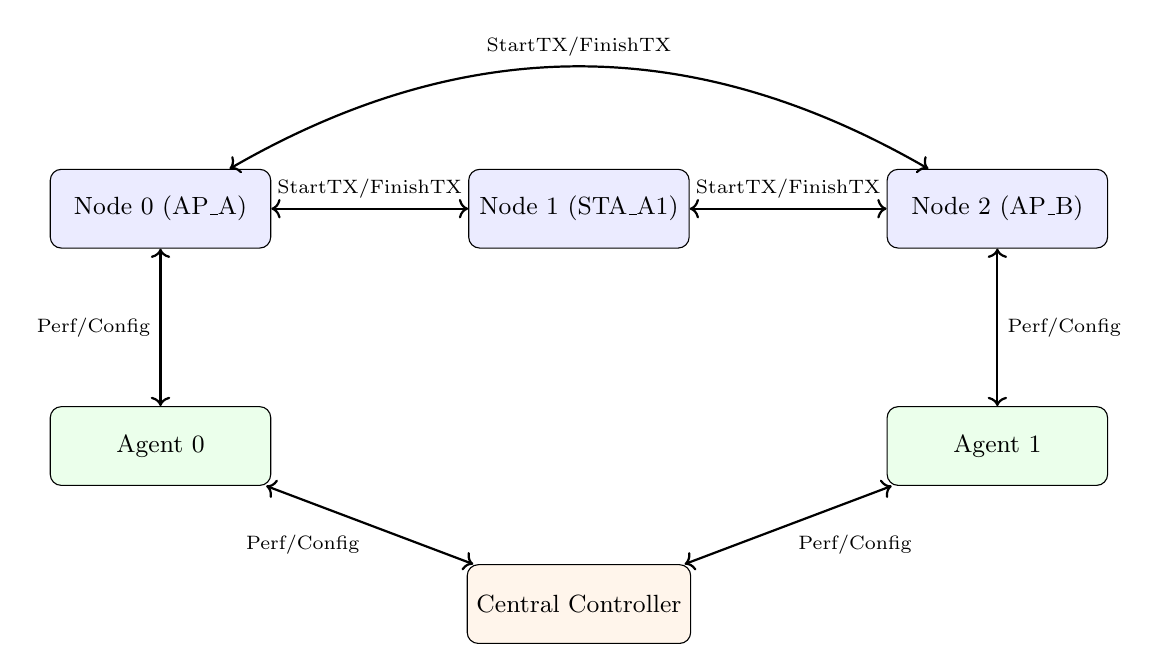
\begin{tikzpicture}[
  box/.style={draw, rounded corners, minimum width=2.8cm, minimum height=1cm,
              fill=blue!8, font=\small},
  arr/.style={-{Stealth[length=6pt]}, thick},
  every node/.style={font=\small}
]
  \node[box] (n1) {Node 0 (AP\_A)};
  \node[box, right=2.5cm of n1] (n2) {Node 1 (STA\_A1)};
  \node[box, right=2.5cm of n2] (n3) {Node 2 (AP\_B)};

  \node[box, fill=green!8, below=2cm of n1] (a1) {Agent 0};
  \node[box, fill=green!8, below=2cm of n3] (a2) {Agent 1};

  \node[box, fill=orange!8, below=1.5cm of $(a1)!0.5!(a2)$] (cc) {Central Controller};

  \draw[arr, <->] (n1) -- node[above]{\scriptsize StartTX/FinishTX} (n2);
  \draw[arr, <->] (n2) -- node[above]{\scriptsize StartTX/FinishTX} (n3);
  \draw[arr, <->, bend left=30] (n1) to node[above]{\scriptsize StartTX/FinishTX} (n3);

  \draw[arr, <->] (n1) -- node[left]{\scriptsize Perf/Config} (a1);
  \draw[arr, <->] (n3) -- node[right]{\scriptsize Perf/Config} (a2);

  \draw[arr, <->] (a1) -- node[below left]{\scriptsize Perf/Config} (cc);
  \draw[arr, <->] (a2) -- node[below right]{\scriptsize Perf/Config} (cc);
\end{tikzpicture}
\caption{Component wiring for a two-BSS scenario with ML agents. Depending on the input, some nodes might not have agents (no learning) and some agents might not be attached to the controller (independent learning).}
\label{fig:wiring}
\end{figure}

% ======================================================================
\section{Components}
\label{sec:components}
% ======================================================================

\subsection{Komondor main}
\label{sec:main}

\texttt{komondor\_main.cc} defines the \texttt{Komondor} compound component, which inherits from \texttt{CostSimEng} and serves as the root of the simulation.  It is instantiated once by \texttt{main()} and owns all other component arrays. \texttt{komondor\_main} extends COST's methods as follows:
\begin{itemize}
    \item \texttt{Setup()} reads \texttt{config\_models}, parses the node CSV (\texttt{GenerateNodesByReadingInputFile}), optionally parses the MAPC CSV (\texttt{GenerateMapcConfiByReadingInputFile}) and the agents CSV (\texttt{GenerateAgents}, \texttt{GenerateCentralController}), pre-computes the received-power matrix, and wires all COST ports.
    \item \texttt{Start()} launches the COST event loop, which triggers the Start() from every instantiated component (nodes, agents, controller).
    \item \texttt{Stop()} collects per-node \texttt{Performance} objects, calls \texttt{ComputeSimulationStatistics}, and writes all output files.
\end{itemize}

To handle the different instantiated components, \texttt{Komondor} holds three COST component arrays (containers) as public members so that port-wiring code can access them:
\begin{itemize}
    \item \texttt{node\_container[]}: one \texttt{Node} per line in the node CSV.
    \item \texttt{traffic\_generator\_container[]}: one \texttt{TrafficGenerator} per node.
    \item \texttt{agent\_container[]} / \texttt{central\_controller[]}: instantiated only when \texttt{-{}-agents} is supplied.
\end{itemize}

When it comes to port wiring---i.e., establishing connections between components, so that they can communicate---,  \texttt{Setup()} establishes the following connection groups:
\begin{itemize}
    \item \textit{Traffic (one-to-one):} A traffic generator component is connected to a node:\\    \texttt{traffic\_generator\_container[n].outportNewPacketGenerated} \\$\to$ \texttt{node\_container[n].InportNewPacketGenerated}.
    \item \textit{Wireless medium (all-to-all):} every node's \texttt{outportSelfStartTX}, \texttt{outportSelfFinishTX}, and \texttt{outportSendLogicalNack} are connected to the corresponding inports of every other node.
    \item \textit{Node (AP) $\leftrightarrow$ Node (STA):} Intra-WLAN MCS request/response and WLAN-configuration update ports are connected between the AP and its associated STAs; spatial-reuse configuration ports are connected within each WLAN.
    \item \textit{Node $\leftrightarrow$ Agent:} When instantiated, agents are connected to nodes to enable the exchange of performance information and commands. \texttt{outportRequestInformationToAp} / \texttt{outportAnswerToAgent} / \texttt{outportSendConfigurationToAp} matched by \texttt{wlan\_code}.
    \item \textit{Agent $\leftrightarrow$ CentralController:} Similarly, agents can be connected to the central controller through \texttt{outportAnswerToController} and \texttt{outportSendCommandToAgent} outports.
\end{itemize}

% ======================================================================

\subsection{The Node Component}
\label{sec:node}

\texttt{Node} (\texttt{Code/main/node.h}) is the central component.  Each \texttt{Node} instance models a single AP (0) or STA (1), indicated as \texttt{node\_type} from the input nodes CSV and implementing the full 802.11 MAC/PHY state machine.

\subsubsection{Inports, Outports, and Timers}

\begin{longtable}{l p{9.5cm}}
\caption{Node interface}\label{tab:node-iface}\\
\toprule
\textbf{Port / Timer} & \textbf{Description} \\
\midrule
\endfirsthead
\toprule
\textbf{Port / Timer} & \textbf{Description} \\
\midrule
\endhead
\bottomrule
\endlastfoot
\multicolumn{2}{l}{\textit{Inports}} \\
\texttt{InportSomeNodeStartTX}      & Another node began transmitting \\
\texttt{InportSomeNodeFinishTX}     & Another node finished transmitting \\
\texttt{InportNackReceived}         & Logical NACK from collision \\
\texttt{InportMCSRequestReceived}   & MCS selection request \\
\texttt{InportMCSResponseReceived}  & MCS selection response \\
\texttt{InportNewPacketGenerated}   & Traffic generator callback \\
\texttt{InportReceivingFromAgent}   & ML agent sends new configuration \\
\midrule
\multicolumn{2}{l}{\textit{Outports}} \\
\texttt{outportSelfStartTX}        & Broadcast ``I started transmitting'' \\
\texttt{outportSelfFinishTX}       & Broadcast ``I finished transmitting'' \\
\texttt{outportSendLogicalNack}    & Send collision NACK \\
\texttt{outportRequestToAgent}     & Request ML decision from agent \\
\texttt{outportAnswerToController}  & Respond to central controller \\
\midrule
\multicolumn{2}{l}{\textit{Timers}} \\
\texttt{trigger\_start\_backoff}   & DIFS/AIFS inter-frame space \\
\texttt{trigger\_end\_backoff}     & Backoff countdown expiration \\
\texttt{trigger\_SIFS}             & SIFS inter-frame space \\
\texttt{trigger\_toFinishTX}       & End of current transmission \\
\texttt{trigger\_ACK\_timeout}     & ACK timeout (retransmission trigger) \\
\texttt{trigger\_CTS\_timeout}     & CTS timeout \\
\texttt{trigger\_DATA\_timeout}    & DATA timeout \\
\texttt{trigger\_NAV\_timeout}     & NAV expiry \\
\texttt{trigger\_inter\_bss\_NAV\_timeout} & Inter-BSS NAV (SR only) \\
\texttt{trigger\_preoccupancy}     & 1\,ps delay before TX occupancy \\
\texttt{trigger\_restart\_sta}     & STA recovery delay \\
\texttt{trigger\_wait\_collisions} & Backoff collision detection \\
\texttt{trigger\_dso\_icr\_timeout}  & DSO ICR wait timer \\
\texttt{trigger\_npca\_switch}       & NPCA radio tuning delay \\
\texttt{trigger\_npca\_backoff}      & NPCA EDCA backoff \\
\texttt{trigger\_npca\_icr\_timeout} & NPCA ICR safety timeout \\
\texttt{trigger\_npca\_timer}        & NPCA switch-back to primary \\
\texttt{trigger\_rho\_measurement}   & Periodic channel utilization sampling \\
\texttt{txop\_sr\_end}               & Spatial reuse TXOP limit \\
\end{longtable}

\subsubsection{Key Member Variables}

\begin{lstlisting}[language=C++,caption={Selected node member variables (simplified)}]
int node_state;                 // Current FSM state
NodeParameters node_params;     // Identity from CSV
Wlan wlan;                      // WLAN membership

// Channel
int primary_channel, current_left_channel, current_right_channel;
double power_received_per_node[];

// Backoff (ChannelAccessState struct)
int current_CW;
double remaining_backoff;
int num_bo_interruptions;

// Transmission
Notification current_notification, rts_notification, cts_notification;

// MAPC
int coordinator_ap_id, mapc_active_group_idx;
int mapc_coordinator_group_rr;
double mapc_txop_data_budget, mapc_txop_per_ap_data_duration;

// Spatial Reuse (SpatialReuseState struct)
struct { int spatial_reuse_enabled, txop_sr_identified, mapc_cosr_active;
         double current_tx_power_sr, non_srg_obss_pd; } sr_state;

// Performance
double throughput, data_packets_sent, data_packets_lost;
\end{lstlisting}

% ======================================================================

\subsection{The TrafficGenerator Component}
\label{sec:traffic}

\texttt{TrafficGenerator} (\texttt{Code/main/traffic\_generator.h}) is a lightweight \texttt{TypeII} component, one instance per node.  It is active only for AP-type nodes (downlink transmissions only), while STAs do not generate traffic independently. A single timer, \texttt{trigger\_new\_packet\_generated}, drives the component.  When it fires, \texttt{GenerateTraffic()} is called: it computes the time until the next packet arrival according to the configured traffic model and re-arms the timer, then fires \texttt{outportNewPacketGenerated()} to notify the associated \texttt{Node}.  The supported models are:

\begin{itemize}
    \item \texttt{TRAFFIC\_POISSON}: exponentially distributed inter-arrival times with mean $1/\lambda$ seconds (\texttt{Exponential(1/traffic\_load)}).
    \item \texttt{TRAFFIC\_DETERMINISTIC}: fixed inter-arrival time.
    \item \texttt{TRAFFIC\_FULL\_BUFFER}: implemented as saturated Poisson ($\lambda = 10^3$~packets/s).
    \item \texttt{TRAFFIC\_FULL\_BUFFER\_NO\_DIFFERENTIATION}: no timer is armed; the node manages its own buffer, which is always virtually full (data packets are generated at the time of initiating a transmission).
\end{itemize}

% ======================================================================

\subsection{The Agent Component}
\label{sec:agent}

\texttt{Agent} (\texttt{Code/main/agent.h}) is a \texttt{TypeII} component that implements the per-WLAN ML pipeline described in Section~\ref{sec:ml}.  One agent is created per WLAN when a \texttt{-{}-agents} CSV is supplied.

The main ports of an agent are as follows:
\begin{itemize}
    \item \textit{Inport} \texttt{InportReceivingInformationFromAp} --- receives a \texttt{Configuration} and \texttt{Performance} snapshot from the AP each time the measurement timer fires.
    \item \textit{Inport} \texttt{InportReceiveCommandFromController} --- receives a command ID, a new configuration, a shared performance value, and an override reward type from the \texttt{CentralController} (centralized mode only).
    \item \textit{Outport} \texttt{outportRequestInformationToAp} --- periodic pull request to the AP.
    \item \textit{Outport} \texttt{outportSendConfigurationToAp} --- pushes the new \texttt{Configuration} computed by the learning algorithm.
    \item \textit{Outport} \texttt{outportAnswerToController} --- forwards the agent's current configuration and performance to the \texttt{CentralController}.
\end{itemize}

Regarding agent timers, \texttt{trigger\_request\_information\_to\_ap} fires at regular intervals of \texttt{time\_between\_requests} seconds, triggering \texttt{RequestInformationToAp()}, which in turn causes the AP to report its \texttt{Performance} back via the inport above.

% ======================================================================

\subsection{The CentralController Component}
\label{sec:cc}

\texttt{CentralController} (\texttt{Code/main/central\_controller.h}) is an optional \texttt{TypeII} component, instantiated at most once per simulation.  It acts as the Collector and Distributor in the centralized ML pipeline: it gathers performance reports from all associated agents, runs a global optimization step, and broadcasts updated configurations back. The main ports of a central controller to interact with agents are:
\begin{itemize}
    \item \textit{Inport} \texttt{InportReceivingInformationFromAgent}: receives an agent ID, the agent's current \texttt{Configuration} and \texttt{Performance}, and the selected action index.
    \item \textit{Outport} \texttt{outportSendCommandToAgent}: sends a command ID and a new \texttt{Configuration} to a specific agent.
\end{itemize}

Regarding timers, the central controller implements the following ones:
\begin{itemize}
    \item \texttt{trigger\_request\_information\_to\_agents}: periodically fires \texttt{RequestInformationToAgents()}, pulling the latest state from every connected agent.
    \item \texttt{trigger\_apply\_ml\_method}: fires \texttt{ApplyMlMethod()}, which invokes the \texttt{MlModel} (wrapping \texttt{CentralizedActionBanning} or a bandit) on the aggregated \texttt{ControllerReport} and dispatches updated configurations.
\end{itemize}

Additional responsibilities include the \texttt{GenerateClusters()} / \texttt{UpdatePerformancePerCluster()} methods, which optionally group WLANs by spatial proximity or interference level, enabling decision-making on a per-cluster basis. \texttt{UpdateControllerReport()} maintains the \texttt{ControllerReport} struct (per-agent action statistics, last configuration, last performance) that serves as input to every ML step.


% ======================================================================
\section{Finite-State Machine}
\label{sec:fsm}
% ======================================================================

The node FSM is the heart of the simulator.  Table~\ref{tab:states} lists every state.

\begin{longtable}{l c p{7.5cm}}
\caption{Node FSM states}\label{tab:states}\\
\toprule
\textbf{Constant} & \textbf{Value} & \textbf{Description} \\
\midrule
\endfirsthead
\toprule
\textbf{Constant} & \textbf{Value} & \textbf{Description} \\
\midrule
\endhead
\bottomrule
\endlastfoot
\multicolumn{3}{l}{\textit{Core 802.11 states}} \\
\texttt{STATE\_SENSING}     & 0  & Idle, sensing medium / backoff countdown \\
\texttt{STATE\_TX\_DATA}    & 1  & Transmitting DATA frame \\
\texttt{STATE\_RX\_DATA}    & 2  & Receiving DATA \\
\texttt{STATE\_WAIT\_ACK}   & 3  & Waiting for ACK after DATA \\
\texttt{STATE\_TX\_ACK}     & 4  & Transmitting ACK \\
\texttt{STATE\_RX\_ACK}     & 5  & Receiving ACK \\
\texttt{STATE\_TX\_RTS}     & 6  & Transmitting RTS \\
\texttt{STATE\_TX\_CTS}     & 7  & Transmitting CTS \\
\texttt{STATE\_RX\_RTS}     & 8  & Receiving RTS \\
\texttt{STATE\_RX\_CTS}     & 9  & Receiving CTS \\
\texttt{STATE\_WAIT\_CTS}   & 10 & Waiting for CTS after RTS \\
\texttt{STATE\_WAIT\_DATA}  & 11 & Waiting for DATA after CTS \\
\texttt{STATE\_NAV}         & 12 & Virtual carrier sense (NAV) \\
\midrule
\multicolumn{3}{l}{\textit{MAPC states}} \\
\texttt{STATE\_TX\_ICF}     & 14 & Transmitting ICF (coordinator) \\
\texttt{STATE\_WAIT\_ICR}   & 15 & Waiting for ICR responses \\
\texttt{STATE\_TX\_TF}      & 16 & Transmitting Trigger Frame \\
\texttt{STATE\_RX\_ICF}     & 17 & Receiving ICF (coordinated AP) \\
\texttt{STATE\_RX\_ICR}     & 18 & Receiving ICR \\
\texttt{STATE\_TX\_ICR}     & 19 & Transmitting ICR \\
\texttt{STATE\_WAIT\_MU\_RTS} & 20 & Waiting for MU-RTS \\
\texttt{STATE\_RX\_MU\_RTS} & 21 & Receiving MU-RTS \\
\texttt{STATE\_WAIT\_TF}    & 22 & Waiting for TF \\
\texttt{STATE\_RX\_TF}      & 23 & Receiving TF \\
\texttt{STATE\_TX\_ACK\_TF} & 24 & Transmitting ACK TF \\
\texttt{STATE\_WAIT\_ACK\_TF} & 25 & Waiting for ACK TF \\
\midrule
\multicolumn{3}{l}{\textit{DSO states}} \\
\texttt{STATE\_TX\_DSO\_ICF}   & 26 & DSO ICF on full BSS bandwidth \\
\texttt{STATE\_RX\_DSO\_ICR}   & 27 & DSO ICR on secondary subband \\
\texttt{STATE\_TX\_DATA\_DSO}  & 28 & DATA on DSO subband \\
\texttt{STATE\_WAIT\_ACK\_DSO} & 29 & Waiting for ACK after DSO DATA \\
\midrule
\multicolumn{3}{l}{\textit{NPCA states}} \\
\texttt{STATE\_TX\_NPCA\_ICF}    & 30 & NPCA ICF on secondary channels \\
\texttt{STATE\_RX\_NPCA\_ICR}    & 31 & AP waiting for NPCA ICR \\
\texttt{STATE\_TX\_DATA\_NPCA}   & 32 & DATA on NPCA secondary channels \\
\texttt{STATE\_WAIT\_ACK\_NPCA}  & 33 & Waiting for ACK after NPCA DATA \\
\texttt{STATE\_TX\_NPCA\_ICR}    & 34 & STA transmitting NPCA ICR \\
\end{longtable}

\subsection{Event Dispatch Architecture}

The two main inport handlers---\texttt{InportSomeNodeStartTX} and \texttt{InportSomeNode\-FinishTX}---dispatch to state-specific handler methods:

\begin{lstlisting}[language=C++,caption={StartTX dispatch (simplified)}]
void Node::InportSomeNodeStartTX(Notification &notification) {
    switch (node_state) {
        case STATE_SENSING:   HandleStartTX_StateSensing(notification); break;
        case STATE_NAV:       HandleStartTX_StateNav(notification);     break;
        case STATE_TX_DATA:   HandleStartTX_StateTxData(notification);  break;
        case STATE_RX_DATA:   HandleStartTX_StateRxData(notification);  break;
        case STATE_WAIT_ACK:  HandleStartTX_StateWaitAck(notification); break;
        case STATE_WAIT_CTS:  HandleStartTX_StateWaitCts(notification); break;
        case STATE_WAIT_DATA: HandleStartTX_StateWaitData(notification); break;
        case STATE_WAIT_ICR:  HandleStartTX_StateWaitIcr(notification); break;
        // ... MAPC/DSO/NPCA states
    }
}
\end{lstlisting}

Similarly, \texttt{InportSomeNodeFinishTX} dispatches to:
\begin{itemize}[nosep]
  \item \texttt{HandleFinishTX\_StateSensing} --- frame ended while idle (processes CTS, ICR, TF, etc.)
  \item \texttt{HandleFinishTX\_StateRxData} --- DATA reception complete (ACK generation)
  \item \texttt{HandleFinishTX\_StateTxData} --- concurrent transmission finished
  \item \texttt{HandleFinishTX\_StateRxIcf}, \texttt{HandleFinishTX\_StateRxIcr}, etc.\ for MAPC states.
\end{itemize}

\subsection{Transmission Flow}

Figure~\ref{fig:txflow} shows the standard four-way handshake (RTS/CTS/DATA/ACK).

\begin{figure}[h]
\centering
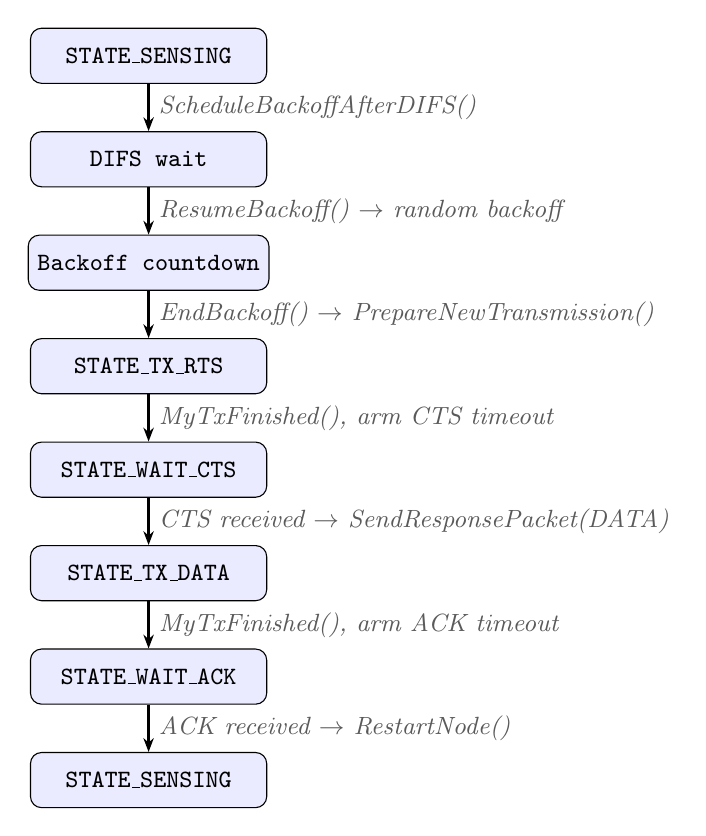
\begin{tikzpicture}[
  state/.style={draw, rounded corners, minimum width=3cm, minimum height=0.7cm,
                fill=blue!8, font=\small\ttfamily},
  act/.style={font=\small\itshape, text=codegray},
  arr/.style={-{Stealth[length=5pt]}, thick},
]
  \node[state] (s0) {STATE\_SENSING};
  \node[state, below=0.6cm of s0] (s1) {DIFS wait};
  \node[state, below=0.6cm of s1] (s2) {Backoff countdown};
  \node[state, below=0.6cm of s2] (s3) {STATE\_TX\_RTS};
  \node[state, below=0.6cm of s3] (s4) {STATE\_WAIT\_CTS};
  \node[state, below=0.6cm of s4] (s5) {STATE\_TX\_DATA};
  \node[state, below=0.6cm of s5] (s6) {STATE\_WAIT\_ACK};
  \node[state, below=0.6cm of s6] (s7) {STATE\_SENSING};

  \draw[arr] (s0) -- node[right, act]{ScheduleBackoffAfterDIFS()} (s1);
  \draw[arr] (s1) -- node[right, act]{ResumeBackoff() $\to$ random backoff} (s2);
  \draw[arr] (s2) -- node[right, act]{EndBackoff() $\to$ PrepareNewTransmission()} (s3);
  \draw[arr] (s3) -- node[right, act]{MyTxFinished(), arm CTS timeout} (s4);
  \draw[arr] (s4) -- node[right, act]{CTS received $\to$ SendResponsePacket(DATA)} (s5);
  \draw[arr] (s5) -- node[right, act]{MyTxFinished(), arm ACK timeout} (s6);
  \draw[arr] (s6) -- node[right, act]{ACK received $\to$ RestartNode()} (s7);
\end{tikzpicture}
\caption{Standard RTS/CTS/DATA/ACK transmission flow.}
\label{fig:txflow}
\end{figure}

Apart from that, other transmission-exchange sequences are defined, thereby granting flexibility to the FSM. The list of sequences is provided in Table~\ref{tab:tx_exchange}.

\begin{longtable}{l l p{5cm}}
\toprule
\textbf{Mode} & \textbf{Frames} & \textbf{Usage} \\
\midrule
No RTS/CTS & DATA $\to$ ACK & Direct short-range TX \\
RTS/CTS & RTS $\to$ CTS $\to$ DATA $\to$ ACK & Standard collision protection \\
Co-TDMA & ICF $\to$ ICR $\to$ [MU-RTS $\to$ DATA $\to$ ACK]$\times N$ & MAPC time-division \\
Co-BF/Co-SR & ICF $\to$ ICR $\to$ TF $\to$ DATA $\to$ ACK\_TF $\to$ ACK & MAPC coordinated BF/SR \\
DSO & DSO\_ICF $\to$ DSO\_ICR $\to$ DATA $\to$ ACK & Dynamic subband \\
NPCA & NPCA\_ICF $\to$ NPCA\_ICR $\to$ DATA $\to$ ACK & Non-primary channel \\
\bottomrule
\caption{Transmission-exchange sequences.}
\label{tab:tx_exchange}
\end{longtable}

\subsection{Interruption Handling}

When a node in \texttt{STATE\_SENSING} receives \texttt{InportSomeNodeStartTX}:
\begin{itemize}[nosep]
  \item \textbf{Own frame} (RTS/CTS/DATA addressed to me): transition to appropriate RX state.
  \item \textbf{Foreign frame above CCA}: freeze backoff, set NAV, transition to \texttt{STATE\_NAV}.
  \item \textbf{Foreign frame below CCA}: ignore (continue backoff).
\end{itemize}

\subsection{Backoff Mechanism}

The backoff subsystem is implemented across two files:
\begin{itemize}[nosep]
  \item \texttt{backoff\_methods.h} --- standalone functions: \texttt{ComputeBackoff()}, \texttt{PickNewCW()}, \texttt{ResetCW()}, \texttt{ComputeEDCABackoff()}.
  \item \texttt{node\_backoff\_methods.h} --- node methods: \texttt{ResumeBackoff()}, \texttt{PauseBackoff()}, \texttt{EndBackoff()}, \texttt{RestartNode()}, \texttt{HandleSlottedBackoffCollision()}.
\end{itemize}

Supported backoff types:
\begin{longtable}{l c l}
\toprule
\textbf{Type} & \textbf{Value} & \textbf{Description} \\
\midrule
\texttt{BACKOFF\_DCF}         & 0 & Standard DCF exponential backoff \\
\texttt{BACKOFF\_EDCA}        & 1 & Per-AC BEB with AIFSN \\
\texttt{BACKOFF\_TOKENIZED}   & 2 & Token-based channel access \\
\texttt{BACKOFF\_DETERMINISTIC} & 3 & Qualcomm deterministic \\
\texttt{BACKOFF\_REPEAT\_BO}  & 4 & Reuse last successful backoff \\
\texttt{BACKOFF\_ECA}         & 5 & Enhanced channel access \\
\texttt{BACKOFF\_SYNCHRONIZED}& 6 & Fixed slot allocation \\
\texttt{BACKOFF\_ML\_ACCESS}  & 7 & ML-learned (external Python server) \\
\bottomrule
\end{longtable}

\texttt{EndBackoff()} is the critical dispatch point: it calls \texttt{PrepareNewTransmission()} (for regular unicast), or initiates MAPC ICF sequences (for coordinator APs), selecting the active group via round-robin:

\begin{lstlisting}[language=C++]
mapc_active_group_idx = mapc_coordinator_group_rr % wlan.num_mapc_groups;
mapc_coordinator_group_rr++;
\end{lstlisting}

% ======================================================================
\subsection{Packet Handling}
\label{sec:packets}
% ======================================================================

\texttt{node\_packet\_methods.h} contains the core transmission logic.

\subsubsection{PrepareNewTransmission()}

Called when a node is ready to transmit.  This method:
\begin{enumerate}[nosep]
  \item Selects the channel bonding width via \texttt{GetTxChannels()}.
  \item Computes A-MPDU aggregation level based on MCS, bandwidth, and TXOP budget.
  \item Sets beamforming weights if applicable (see Section~\ref{sec:bf}).
  \item Calls \texttt{GenerateNotification()} to build the \texttt{Notification} struct.
\end{enumerate}

\subsubsection{GenerateNotification()}

Populates a \texttt{Notification} with all \texttt{TxInfo} fields: source/destination IDs, packet type, channel range, TX power, NAV time, MCS, beamforming parameters, MAPC fields, and spatial-reuse state. If spatial reuse is active (\texttt{sr\_state.mapc\_cosr\_active} or legacy SR), the reduced TX power from \texttt{sr\_state.current\_tx\_power\_sr} is used instead of the default.

\subsubsection{StartTransmission()}

Fires \texttt{outportSelfStartTX(notification)}, which broadcasts to all other nodes.  A critical ordering constraint: \texttt{STATE\_TX\_TF} must be checked \emph{before} the \texttt{exchange\_sequence} check, because TF is sent mid-sequence while the first frame type is still ICF.

\subsubsection{MyTxFinished()}

Handles the \texttt{trigger\_toFinishTX} event for every TX state.  Broadcasts a finish notification via \texttt{outportSelfFinishTX()}, then transitions to the appropriate next state (e.g., \texttt{STATE\_WAIT\_ACK} after DATA, \texttt{STATE\_SENSING} after ACK).

\subsubsection{SendResponsePacket()}

The SIFS timer handler.  Generates and sends response frames: ACK (after DATA), CTS (after RTS), ICR (after ICF), or NPCA-ICR, depending on \texttt{node\_state}.

\subsubsection{Timeout Handlers}

Defined in \texttt{node\_timeout\_methods.h}:
\begin{itemize}[nosep]
  \item \texttt{AckTimeout()} --- No ACK received; Modify channel access parameters (e.g., increment CW), retry or drop the frame.
  \item \texttt{CtsTimeout()} --- No CTS after RTS; modify channel access parameters (e.g., increment CW), retry.
  \item \texttt{DataTimeout()} --- No DATA after CTS sent; return to sensing.
  \item \texttt{NpcaIcrTimeout()} --- Safety fallback if no NPCA ICR is received.
\end{itemize}

% ======================================================================
\section{Data Structures}
\label{sec:structs}
% ======================================================================

\subsection{NodeParameters}

Per-node configuration loaded from the node CSV.

\begin{lstlisting}[language=C++,caption={NodeParameters (key fields)}]
struct NodeParameters {
    int node_id;
    int node_type;             // NODE_TYPE_AP (0), NODE_TYPE_STA (1)
    char wlan_code[20];
    double x, y, z;            // Position (meters)
    int primary_channel;
    int min_channel_allowed, max_channel_allowed;
    int channel_bonding_model;
    double tx_power_default;   // dBm
    double cca_default;        // dBm
    int traffic_model;
    int ieee_protocol;
};
\end{lstlisting}

\subsection{Wlan}

WLAN-level configuration grouping an AP and its associated STAs.

\begin{lstlisting}[language=C++,caption={Wlan (key fields)}]
struct Wlan {
    int wlan_id;
    char wlan_code[20];
    int ap_id;
    int num_stas;
    int *list_sta_id;

    // MAPC (up to MAX_MAPC_GROUPS_PER_WLAN = 8)
    int mapc_enabled, num_mapc_groups;
    int mapc_group_ids[8], mapc_method_ids[8];
    int *mapc_peer_ap_ids[8];
    int FindMapcGroupIdx(int group_id);

    // Beamforming
    int bf_enabled, bf_N_elements;
    double bf_d_spacing, bf_az_deg;

    // DSO / NPCA / EDCA / SR ...
};
\end{lstlisting}

\subsection{Notification and TxInfo}

The message passed between nodes on every transmission event.

\begin{lstlisting}[language=C++,caption={TxInfo (key fields)}]
struct TxInfo {
    int packet_type, source_id, destination_id;
    int left_channel, right_channel;
    double tx_power, nav_time;
    double data_duration, ack_duration, rts_duration, cts_duration;
    int bits_ofdm_sym, modulation, num_packets_aggregated;

    // Beamforming
    int beamforming_active, beam_N_elements, beam_num_nulls, beam_use_zf;
    double beam_d_spacing, beam_az_main_rad;
    double beam_null_az_rad[MAX_BEAM_NULLS];

    // MAPC
    int mapc_group_id;
    double mapc_allocated_data_duration, mapc_sr_peer_tx_power;

    // Spatial Reuse
    int srg_obss_pd;
    double non_srg_obss_pd;

    // Preamble puncturing
    int punctured_channels[MAX_CHANNELS];
};

struct Notification {
    TxInfo tx_info;
    double timestamp;
};
\end{lstlisting}

\subsection{Performance}

Reported from Node to Agent at the end of each measurement window.

\begin{lstlisting}[language=C++]
struct Performance {
    double throughput, max_bound_throughput;
    double data_packets_sent, data_packets_lost;
    double rts_cts_sent, rts_cts_lost;
    double num_tx_init_not_possible;
    double average_delay, max_delay, min_delay;
    double average_utilization;
    double successful_channel_occupancy;
    double *rssi_list;            // Per-WLAN RSSI (pW)
};
\end{lstlisting}

\subsection{Configuration and Action}

\begin{lstlisting}[language=C++]
struct Configuration {
    double timestamp;
    int selected_primary_channel;
    double selected_pd;           // pW
    double selected_tx_power;     // pW
    int selected_max_bandwidth;   // num channels
    int spatial_reuse_enabled;
    double non_srg_obss_pd;       // pW
};

struct Action {
    int id, channel;
    double cca, tx_power;         // pW
    int max_bandwidth;
    double instantaneous_reward, cumulative_reward;
    int times_played;
};
\end{lstlisting}

% ======================================================================
\section{Channel and Power Model}
\label{sec:channel}
% ======================================================================

\texttt{power\_channel\_methods.h} implements the PHY-layer abstractions.

\subsection{Path Loss and Received Power}

\texttt{ComputePowerReceived()} computes the power received at a given distance using configurable path-loss models (free-space, log-distance, IEEE~802.11ax indoor, etc.).  The received-power matrix is pre-computed at simulation start to save computation time, but it is updated upon specific events (e.g., changes in transmission power or position).

\subsection{SINR Computation}

\texttt{ComputeSINR()} sums interference from all concurrently active transmitters on overlapping channels:

\[
  \text{SINR} = \frac{P_{\text{signal}}}{N_0 + \sum_{i \in \mathcal{I}} P_{\text{interference},i}}
\]

\subsection{Channel Bonding}

\texttt{GetTxChannels()} implements multiple channel-bonding models:

\begin{longtable}{l c p{6.5cm}}
\toprule
\textbf{Model} & \textbf{Value} & \textbf{Description} \\
\midrule
\texttt{CB\_ONLY\_PRIMARY}        & 0 & Primary channel only (20\,MHz) \\
\texttt{CB\_ALWAYS\_MAX}          & 2 & Use all channels if all are free \\
\texttt{CB\_ALWAYS\_MAX\_LOG2}    & 3 & Widest contiguous power-of-2 bandwidth \\
\texttt{CB\_PREAMBLE\_PUNCTURING} & 6 & Allow punctured subchannels \\
\bottomrule
\end{longtable}

\texttt{GetTxChannelsNPCA()} is the NPCA variant that checks secondary channels for non-primary channel access operation.

\subsection{Power Sensing Update}

\texttt{UpdatePowerSensedPerNode()} updates per-node power tracking when a new transmission starts.  It takes receiver coordinates (\texttt{rx\_x, rx\_y, rx\_z}) and multiplies \texttt{pw\_received} by the beamforming gain---but \emph{only for DATA frames}:

\begin{lstlisting}[language=C++]
if (notification.packet_type == PACKET_TYPE_DATA) {
    double bf_gain = ComputeRxBeamGain(tx_info, tx_x, tx_y, rx_x, rx_y);
    pw_received *= bf_gain;
}
\end{lstlisting}

Control frames (ICF, TF, RTS, CTS, ACK) remain omnidirectional to prevent coordination deadlocks.

% ======================================================================
\section{Beamforming}
\label{sec:bf}
% ======================================================================

\texttt{beamforming\_methods.h} implements horizontal Uniform Linear Array (ULA) beamforming with two null-placement algorithms.

\subsection{Array Model}

The phase shift for element $n$ steering toward azimuth $\theta$ is:
\[
  \phi_n = \exp\!\bigl(j \cdot 2\pi \cdot d \cdot n \cdot \sin(\theta)\bigr)
\]
where $d$ is the element spacing in wavelengths.

\subsection{Algorithms}

\begin{description}[style=nextline]
  \item[\texttt{ComputeBeamWeights()} --- Projection Null-Steerer (Gram--Schmidt)]
  Used for standalone beamforming.  Steers the main beam and places nulls via Gram--Schmidt orthogonalization.  Set \texttt{beam\_use\_zf = 0}.

  \item[\texttt{ComputeZFBeamWeights()} --- Zero-Forcing Precoding]
  Used for Co-BF (coordinated beamforming).  Computes $\mathbf{w} = \mathbf{H}(\mathbf{H}^H \mathbf{H})^{-1} \mathbf{e}_1$, guaranteeing exact simultaneous nulls.  Includes \texttt{SolveComplexLinearSystem()} (Gaussian elimination with partial pivoting, max $5 \times 5$).  Set \texttt{beam\_use\_zf = 1}.
\end{description}

\texttt{ComputeRxBeamGain()} returns the beam gain at the receiver's angle.

\subsection{Integration with Transmission}

In \texttt{PrepareNewTransmission()}:
\begin{itemize}[nosep]
  \item \textbf{Standalone BF}: projection null-steerer, \texttt{beam\_use\_zf = 0}.
  \item \textbf{Co-BF coordinator}: ZF with nulls toward peer STAs, \texttt{beam\_use\_zf = 1}.
  \item \textbf{Co-BF coordinated AP}: ZF with null toward coordinator's STA.
  \item \textbf{Co-TDMA / Co-SR}: projection if BF enabled, \texttt{beam\_use\_zf = 0}.
\end{itemize}

\textbf{Constraints}: \texttt{BF\_MAX\_N\_ELEMENTS = 32} (stack arrays).  ZF fallback to projection if $N < K+1$ or $K+1 > \texttt{MAX\_ZF\_CONSTRAINTS}\ (5)$.

% ======================================================================
\section{Backoff models}
\label{sec:backoff}
% ======================================================================

Different backoff types are implemented (see Table~\ref{tab:backoff_types}).

\begin{longtable}{l c l}
\toprule
\textbf{Type} & \textbf{Value} & \textbf{Description} \\
\midrule
\texttt{BACKOFF\_DCF}         & 0 & Standard DCF exponential backoff \\
\texttt{BACKOFF\_EDCA}        & 1 & Per-AC BEB with AIFSN \\
\texttt{BACKOFF\_TOKENIZED}   & 2 & Token-based channel access \\
\texttt{BACKOFF\_DETERMINISTIC} & 3 & Qualcomm deterministic \\
\texttt{BACKOFF\_REPEAT\_BO}  & 4 & Reuse last successful backoff \\
\texttt{BACKOFF\_ECA}         & 5 & Enhanced channel access \\
\texttt{BACKOFF\_SYNCHRONIZED}& 6 & Fixed slot allocation \\
\bottomrule
\caption{Backoff types.}
\label{tab:backoff_types}
\end{longtable}

In \texttt{BACKOFF\_DCF} and \texttt{BACKOFF\_EDCA}, the contention window follows binary exponential backoff, whereby the contention window (CW) is updated upon experiencing packet losses:
\[
  \text{CW}_{\text{new}} = \min(2 \cdot \text{CW}_{\text{current}} + 1, \ \text{CW}_{\text{max}})
\]
On successful transmission, \texttt{CW} resets to \texttt{CW\_min}.

EDCA differentiates traffic into four Access Categories (AC):

\begin{longtable}{l l l}
\toprule
\textbf{AC} & \textbf{Traffic} & \textbf{Typical CW} \\
\midrule
\texttt{AC\_VO} (0) & Voice      & [8, 16] \\
\texttt{AC\_VI} (1) & Video      & [16, 32] \\
\texttt{AC\_BE} (2) & Best Effort & [32, 1024] \\
\texttt{AC\_BK} (3) & Background & [32, 1024] \\
\bottomrule
\end{longtable}

Each AC has its own contention window bounds (\texttt{ac\_cw\_min[]}, \texttt{ac\_cw\_max[]}), arbitration inter-frame spacing (\texttt{ac\_aifsn[]}), and TXOP limit (\texttt{ac\_txop\_limit[]}).
\texttt{ComputeEDCABackoff()} in \texttt{backoff\_methods.h} applies the per-AC AIFSN and CW parameters.

% ======================================================================
\section{Multi-AP Coordination (MAPC)}
\label{sec:mapc}
% ======================================================================

MAPC enables coordinated operation between multiple BSSs.\footnote{Wilhelmi, F., Bellalta, B., Geraci, G., Galati-Giordano, L., Meneghello, F., Kijanka, A., Val, I., \& López-Pérez, D. (2026). A Tutorial on IEEE 802.11 bn Multi-AP Coordination for Wi-Fi 8: From Standardization to Performance Evaluation. arXiv preprint arXiv:2606.13759.}  Three methods are supported:

\begin{longtable}{l c p{7cm}}
\toprule
\textbf{Method} & \textbf{Constant} & \textbf{Description} \\
\midrule
Co-TDMA & \texttt{MAPC\_CO\_TDMA} (1) & Time-division among coordinated APs \\
Co-SR   & \texttt{MAPC\_CO\_SR} (2)   & Coordinated spatial reuse with power adaptation \\
Co-BF   & \texttt{MAPC\_CO\_BF} (3)   & Coordinated beamforming with ZF nulls \\
\bottomrule
\end{longtable}

\subsection{Frame Exchange Sequence}

\begin{figure}[h]
\centering
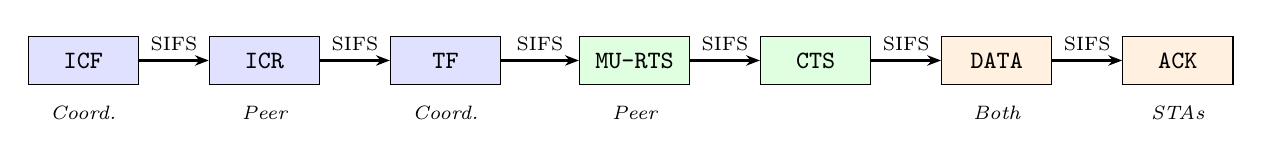
\begin{tikzpicture}[
  frame/.style={draw, minimum width=1.4cm, minimum height=0.6cm, font=\small\ttfamily, fill=#1},
  frame/.default=blue!12,
  arr/.style={-{Stealth[length=5pt]}, thick},
  lbl/.style={font=\scriptsize, midway, above},
]
  \node[frame] (icf) at (0,0) {ICF};
  \node[frame] (icr) at (2.3,0) {ICR};
  \node[frame] (tf)  at (4.6,0) {TF};
  \node[frame=green!12] (mrts) at (7.0,0) {MU-RTS};
  \node[frame=green!12] (cts)  at (9.3,0) {CTS};
  \node[frame=orange!12] (data) at (11.6,0) {DATA};
  \node[frame=orange!12] (ack) at (13.9,0) {ACK};

  \draw[arr] (icf) -- node[lbl]{SIFS} (icr);
  \draw[arr] (icr) -- node[lbl]{SIFS} (tf);
  \draw[arr] (tf) -- node[lbl]{SIFS} (mrts);
  \draw[arr] (mrts) -- node[lbl]{SIFS} (cts);
  \draw[arr] (cts) -- node[lbl]{SIFS} (data);
  \draw[arr] (data) -- node[lbl]{SIFS} (ack);

  \node[below=0.15cm of icf, font=\scriptsize\itshape] {Coord.};
  \node[below=0.15cm of icr, font=\scriptsize\itshape] {Peer};
  \node[below=0.15cm of tf, font=\scriptsize\itshape] {Coord.};
  \node[below=0.15cm of mrts, font=\scriptsize\itshape] {Peer};
  \node[below=0.15cm of data, font=\scriptsize\itshape] {Both};
  \node[below=0.15cm of ack, font=\scriptsize\itshape] {STAs};
\end{tikzpicture}
\caption{MAPC Co-TDMA frame exchange.}
\label{fig:mapc}
\end{figure}

\begin{enumerate}[nosep]
  \item \textbf{ICF} (Initial Control Frame): Coordinator broadcasts to its MAPC group (\texttt{destination\_id = NODE\_ID\_MAPC\_BROADCAST}).
  \item \textbf{ICR} (ICF Response): Coordinated APs acknowledge readiness.
  \item \textbf{TF} (Trigger Frame): Coordinator allocates time slots.
  \item \textbf{MU-RTS}: Coordinated AP solicits CTS from its STA.
  \item \textbf{CTS / DATA / ACK}: Per-AP data exchange within the allocated TXOP.
\end{enumerate}

\subsection{Multi-Group Support}

Each WLAN can participate in up to \texttt{MAX\_MAPC\_GROUPS\_PER\_WLAN}~(8) groups.  The \texttt{Wlan} struct stores per-group arrays: \texttt{mapc\_group\_ids[]}, \texttt{mapc\_method\_ids[]}, \texttt{mapc\_peer\_ap\_ids[]}, etc.  The coordinator round-robins through groups via \texttt{mapc\_coordinator\_group\_rr}, but other implementations are possible.

\subsection{Co-TDMA TXOP Split}

In Co-TDMA, the coordinator AP divides the TXOP equally among active APs as a baseline implementation. In \texttt{ProceedAfterIcr()}: $\text{per\_ap\_duration} = (\text{TXOP}_{\max} - \text{overhead}) / N_{\text{active}}$, embedded in \texttt{mapc\_allocated\_data\_duration} of the TF notification.

\subsection{Co-SR Power Computation}

In the baseline implementation of Co-SR, \texttt{ComputeCoSRTxPowers()} returns the pre-configured power from \texttt{wlan.mapc\_sr\_tx\_power\_dbm[group\_idx]}, which is indicated by the user through the MAPC input file. The coordinator sets \texttt{sr\_state.mapc\_cosr\_active = TRUE} and embeds the peer's allocated power in \texttt{tf\_notification.tx\_info.mapc\_sr\_peer\_tx\_power}.

% ======================================================================
\section{NPCA and DSO}
\label{sec:npca}
% ======================================================================

\subsection{DSO (Dynamic Subband Operation)}

DSO allows a BSS to use a secondary subband after winning contention on the primary.  The flow is:
\begin{enumerate}[nosep]
  \item AP sends DSO\_ICF (non-HT duplicate on full BSS bandwidth).
  \item Timer-modeled ICR response on secondary subband.
  \item DATA transmission on the DSO secondary subband.
  \item Primary channel is freed during DATA.
\end{enumerate}
Timing overhead: $\sim$136\,$\mu$s (ICF + switch + ICR + SIFS).

\subsection{NPCA (Non-Primary Channel Access)}

NPCA allows a BSS to access secondary channels without contending on the primary. The operation works as follows:

\begin{enumerate}[nosep]
  \item AP detects inter-BSS PPDU on primary, freezes primary backoff.
  \item AP switches to the NPCA primary channel, which takes a switch time delay (set to 16$\mu$s by default). 
  \item AP sends NPCA ICF on the NPCA primary channel (\texttt{STATE\_TX\_NPCA\_ICF}).
  \item STA detects ICF finish in \texttt{HandleFinishTX\_StateSensing} (guard: \texttt{npca\_enabled \&\& npca\_primary\_channel >= 0 \&\& node\_type != AP}).
  \item STA sends ICR after SIFS (\texttt{STATE\_TX\_NPCA\_ICR}).
  \item AP receives ICR in \texttt{InportSomeNodeFinishTX} case \texttt{STATE\_RX\_NPCA\_ICR}.
  \item AP cancels safety timeout and begins DATA transmission (\texttt{STATE\_TX\_DATA\_NPCA}).
  \item AP returns to the primary channel, which again takes a switch time delay.
\end{enumerate}

A safety timeout (SIFS + switch time + ICR duration $\approx 52\,\mu$s) is kept as a fallback but fires 0~times in validated scenarios.

% ======================================================================
\section{Machine Learning Subsystem}
\label{sec:ml}
% ======================================================================

The ML subsystem enables online parameter tuning through a modular pipeline. A node (AP) can have an associated agent running a certain ML algorithm (e.g., MABs with $\varepsilon$-greedy) to do a certain operation (e.g., joint channel and transmission power optimization). Agents can be associated with a central controller (optional), which may centralize the optimization operation.

\begin{figure}[h]
\centering
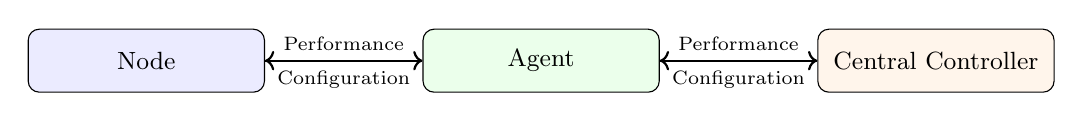
\begin{tikzpicture}[
  box/.style={draw, rounded corners, minimum width=3cm, minimum height=0.8cm,
              fill=#1, font=\small},
  box/.default=blue!8,
  arr/.style={-{Stealth[length=5pt]}, thick},
]
  \node[box]                   (node)  {Node};
  \node[box=green!8, right=2cm of node]  (agent) {Agent};
  \node[box=orange!8, right=2cm of agent] (cc)    {Central Controller};

  \draw[arr, ->] (node) -- node[above, font=\scriptsize]{Performance} (agent);
  \draw[arr, <-] (node) -- node[below, font=\scriptsize]{Configuration} (agent);
  \draw[arr, ->] (agent) -- node[above, font=\scriptsize]{Performance} (cc);
  \draw[arr, <-] (agent) -- node[below, font=\scriptsize]{Configuration} (cc);
\end{tikzpicture}
\caption{ML subsystem architecture.}
\label{fig:ml}
\end{figure}

\subsection{Agent's Flow}

In \texttt{Agent::ComputeNewConfiguration()}:
\begin{enumerate}[nosep]
  \item \texttt{arm\_ix = pre\_processor.EncodeConfiguration(config, from\_ap)} --- current config $\to$ action index.
  \item \texttt{reward = pre\_processor.ComputeReward(type, performance)} --- performance $\to$ scalar reward.
  \item \texttt{ml\_output = learning\_algorithm.Update(arm\_ix, reward, available\_arms)} --- get new action.
  \item \texttt{pre\_processor.DecodeAction(ml\_output, \&new\_config)} --- action $\to$ new configuration.
  \item \texttt{outportSendToNode(new\_config)} --- apply to node.
\end{enumerate}

\subsection{Learning Algorithms}

\begin{description}[style=nextline]
  \item[Multi-Armed Bandits (\texttt{multi\_armed\_bandits.h})]
  Three strategies: $\varepsilon$-greedy, UCB1 (Upper Confidence Bound), and Thompson Sampling (Beta distributions).  Action space is the Cartesian product of channels $\times$ CCA values $\times$ power levels $\times$ sensitivity levels.

  \item[RTOT (\texttt{rtot\_algorithm.h})]
  Recommended TX Output Threshold.  Adjusts \texttt{non\_srg\_obss\_pd} with a step-size, bounded by $[\text{min}, \text{max}]$.  Direction reverses when reward decreases.  Note: \texttt{ml\_output} is \texttt{double} (not \texttt{int}) to handle RTOT's continuous output correctly.

  \item[External Model (\texttt{external\_model\_client.h})]
  Socket communication with an external Python ML server.  C++ sends state vector (\texttt{uint32\_t n\_feat}, then \texttt{n\_feat $\times$ float32}), receives action vector.  Enables DRL and other advanced algorithms.
\end{description}

\subsection{Reward Types}

\begin{longtable}{c l l}
\toprule
\textbf{Value} & \textbf{Constant} & \textbf{Formula} \\
\midrule
1 & \texttt{REWARD\_TYPE\_PACKETS\_SUCCESSFUL} & (sent $-$ lost) / sent \\
2 & \texttt{REWARD\_TYPE\_AVERAGE\_THROUGHPUT} & throughput / max\_bound \\
3 & \texttt{REWARD\_TYPE\_MIN\_RSSI} & min(rssi\_per\_sta) \\
4 & \texttt{REWARD\_TYPE\_MAX\_DELAY} & 1.0 / max\_delay \\
5 & \texttt{REWARD\_TYPE\_MIN\_DELAY} & 1.0 / min\_delay \\
6 & \texttt{REWARD\_TYPE\_AVERAGE\_DELAY} & 1.0 / average\_delay \\
7 & \texttt{REWARD\_TYPE\_CHANNEL\_OCCUPANCY} & successful\_ch\_occupancy \\
\bottomrule
\end{longtable}

\subsection{External ML Server Integration}

Python servers in \texttt{Code/learning\_modules/python\_servers/}:
\begin{itemize}[nosep]
  \item \texttt{ml\_server\_passthrough.py} --- Smoke-test: echoes arm index unchanged.
  \item \texttt{ml\_server\_pytorch.py} --- PyTorch JIT inference with DQN training hook.
  \item \texttt{ml\_server\_random.py} --- Baseline random action selection.
\end{itemize}

Wire protocol: C++ sends \texttt{[uint32 n\_feat][n\_feat $\times$ float32]}, Python returns \texttt{[float32 action]}.

\subsection{Central Controller}

\texttt{CentralController} (\texttt{central\_controller.h}) coordinates multi-WLAN learning.  It receives configurations from all agents, can ban/allow actions via \texttt{CentralizedActionBanning}, and distributes coordinated commands.

% ======================================================================
\section{Input Configuration}
\label{sec:input}
% ======================================================================

All scenarios are defined through semicolon-delimited CSV files.

\subsection{Node CSV}

Each row defines one node (AP or STA).  Key columns:

\begin{longtable}{c l p{6cm}}
\toprule
\textbf{Col} & \textbf{Field} & \textbf{Description} \\
\midrule
\endfirsthead
\toprule
\textbf{Col} & \textbf{Field} & \textbf{Description} \\
\midrule
\endhead
\bottomrule
\endlastfoot
0  & \texttt{node\_code}             & Identifier (AP\_A, STA\_B1, etc.) \\
1  & \texttt{node\_type}             & 0 = AP, 1 = STA \\
2  & \texttt{wlan\_code}             & WLAN identifier (string, e.g.\ ``A'') \\
3--5  & \texttt{x, y, z}            & Position in meters \\
6  & \texttt{central\_freq}          & Center frequency (GHz) \\
7  & \texttt{cb\_model}              & Channel bonding model \\
8  & \texttt{primary\_channel}       & Primary channel index \\
9--10 & \texttt{min/max\_channel}    & Allowed channel range \\
11 & \texttt{tx\_power}              & TX power (dBm) \\
12 & \texttt{sensitivity}            & Receiver sensitivity (dBm) \\
13 & \texttt{traffic\_model}         & Traffic generation model \\
14 & \texttt{traffic\_load}          & Packet generation rate \\
\ldots & \ldots & (backoff, CW, RTS/CTS, BSS color, SR, \ldots) \\
28--31 & \texttt{bf\_enabled, bf\_N, bf\_d, bf\_az\_deg} & Beamforming config (optional) \\
37 & \texttt{dso\_enabled}           & DSO enable (0/1) \\
38 & \texttt{npca\_enabled}          & NPCA enable (0/1) \\
39 & \texttt{npca\_primary\_ch}      & NPCA primary channel \\
\end{longtable}

\subsection{MAPC CSV}

\begin{lstlisting}[language=CSV,caption={MAPC configuration format}]
GroupID;Method;CoordinatedBSSIds;ExtraParams
1;CO_TDMA;A,B;
2;CO_SR;B,C;20.0
\end{lstlisting}

\begin{itemize}[nosep]
  \item \texttt{GroupID}: Integer group identifier.
  \item \texttt{Method}: \texttt{CO\_TDMA}, \texttt{CO\_SR}, or \texttt{CO\_BF}.
  \item \texttt{CoordinatedBSSIds}: Comma-separated WLAN codes (string matching).
  \item \texttt{ExtraParams}: Method-specific (e.g., TX power in dBm for Co-SR).
\end{itemize}

\subsection{Agent CSV}

Each row defines one ML agent.  Key columns: \texttt{wlan\_code}, \texttt{centralized} (0/1), \texttt{time\_between\_requests} (seconds), \texttt{actions channels}, \texttt{actions cca} (dBm, comma-separated), \texttt{actions tx power} (dBm, comma-separated), \texttt{max\_bandwidth}, \texttt{reward} (type constant), \texttt{learning mechanism}, \texttt{selected\_strategy}.

\subsection{Example Run}

\begin{lstlisting}[language=bash,caption={Running a simulation}]
cd Code/main
./komondor_main \
    --nodes ../input/examples/basic_examples/input_nodes.csv \
    --time 10.0 \
    --seed 1

# With agents:
./komondor_main \
    --nodes ../input/examples/basic_examples/input_nodes.csv \
    --agents ../input/examples/basic_examples/agents.csv \
    --time 10.0 --seed 1

# With MAPC:
./komondor_main \
    --nodes ../input/examples/mapc_example/input_nodes_mapc_example.csv \
    --mapc ../input/examples/mapc_example/mapc_cotdma_example.csv \
    --time 10.0 --seed 1

\end{lstlisting}

% ======================================================================
\section{Output}
\label{sec:output}
% ======================================================================

Simulation results are written to \texttt{Code/output/} and include per-node statistics:

\begin{itemize}[nosep]
  \item Throughput (Mbps)
  \item Packets sent / lost / ACKed
  \item Average, min, max delay
  \item Channel utilization and occupancy
  \item RSSI and SINR measurements
  \item Spatial reuse and MAPC performance metrics
\end{itemize}

The output formatting is handled by \texttt{output\_methods.h}, invoked from \texttt{komondor\_main.cc} after the simulation completes.  Per-node log files are written if \texttt{save\_node\_logs} is enabled, using the \texttt{LOGS()} macro:

\begin{lstlisting}[language=C++]
LOGS(save_node_logs, node_logger.file, "%.15f;N%d;%s;%s\n",
     SimTime(), node_params.node_id, "StartTX", "DATA");
\end{lstlisting}

% ======================================================================
\section{Coding Conventions}
\label{sec:conventions}
% ======================================================================

\begin{itemize}[nosep]
  \item \textbf{C++98 strict}: No C++11 features.  No \texttt{auto}, no lambdas, no in-class member initializers, no range-based for, no \texttt{nullptr}.  Use \texttt{NULL}, constructor initializer lists, and explicit type declarations.
  \item \textbf{Tabs} for indentation (not spaces).
  \item \textbf{Method signatures}: \texttt{void Node :: MethodName(...)} with spaces around \texttt{::}.
  \item \textbf{LOGS macro}: \texttt{LOGS(save\_node\_logs, node\_logger.file, ...)} --- always preserve when editing.
  \item \textbf{Header-only}: almost all logic in \texttt{.h} files.  The COST preprocessor requires this for component methods.
  \item \textbf{Constants}: all-caps macros in \texttt{list\_of\_macros.h} (e.g., \texttt{STATE\_SENSING}, \texttt{PACKET\_TYPE\_DATA}).
  \item \textbf{loss\_reason}: a member variable (not local).
  \item \textbf{nav\_collision} / \textbf{inter\_bss\_nav\_collision}: local variables declared inside each handler.
\end{itemize}

% ======================================================================
\section{Adding a New Feature: Checklist}
\label{sec:checklist}
% ======================================================================

When adding a new feature to Komondor, follow this checklist:

\begin{enumerate}
  \item \textbf{Define constants} in \texttt{list\_of\_macros.h} (new states, packet types, default values).
  \item \textbf{Extend structures} in \texttt{Code/structures/} if new per-node, per-WLAN, or per-notification fields are needed.
  \item \textbf{Add CSV columns} and parsing logic in \texttt{input\_loader.h}.  Use \texttt{GetField()} with null-checks for backward compatibility.
  \item \textbf{Implement logic} in the appropriate \texttt{Code/methods/} header file.
  \item \textbf{Wire into the FSM} by adding cases to the \texttt{HandleStartTX\_*} / \texttt{HandleFinishTX\_*} dispatch in \texttt{node.h}.
  \item \textbf{Handle timer events} by adding new timers in \texttt{node.h} and their handlers in \texttt{node\_timeout\_methods.h} or \texttt{node\_backoff\_methods.h}.
  \item \textbf{Initialize} new member variables in \texttt{InitializeVariables()} and reset them in \texttt{RestartNode()}.
  \item \textbf{Create test scenarios} in \texttt{Code/input/validation/}.
  \item \textbf{Structural verification}: Use a brace-counting script to verify \texttt{node.h} integrity after any switch-case modifications (expected depth = 4 at EOF due to outer component block).
\end{enumerate}

% ======================================================================
\section{Common Pitfalls}
\label{sec:pitfalls}
% ======================================================================

Lessons learned from the refactoring history:

\begin{enumerate}
  \item \textbf{Function extraction}: When extracting a code block into a helper, the original body \emph{must} be removed from the call site.  Leaving both causes double execution (double buffer fill, double trigger firings, double stats counting).

  \item \textbf{Broadcast frame destination}: ICF and TF use \texttt{NODE\_ID\_MAPC\_BROADCAST (-2)}, not a specific node ID.  Finish notifications must preserve this value.

  \item \textbf{BF on control frames}: Beamforming gain must be DATA-only.  Applying BF to control frames (ICF, RTS, CTS, ACK) causes coordination deadlocks because ULA nulls can zero out control-frame power.

  \item \textbf{Integer truncation}: The RTOT algorithm returns a \texttt{double} (power in pW).  Casting to \texttt{int} gives 0.  Use \texttt{double} throughout the ML pipeline.

  \item \textbf{\texttt{atoi()} on string codes}: \texttt{atoi("A") = atoi("B") = 0}.  Use \texttt{std::string} comparison for WLAN codes.

  \item \textbf{NAV time in ICF handler}: The coordinated AP's ICF handler copies duration fields but historically missed \texttt{nav\_time}.  Third-party APs crash if \texttt{nav\_time = 0}.

  \item \textbf{StartTX TF ordering}: \texttt{STATE\_TX\_TF} must be checked before the \texttt{exchange\_sequence} check in \texttt{StartTransmission()}.

  \item \textbf{Python patch scripts}: A \texttt{sys.exit(1)} on any failed patch aborts before the file write, losing all in-memory patches.  Split into per-file scripts.

  \item \textbf{C++98 constraints}: No \texttt{auto}, no lambdas, no in-class initializers, no range-based for loops.  Use \texttt{NULL}, constructor initializer lists, and explicit type declarations.

\end{enumerate}

% ======================================================================
\section{Quick Reference: Key Methods}
\label{sec:reference}
% ======================================================================

\begin{longtable}{p{5.5cm} p{2.5cm} p{6cm}}
\caption{Key methods quick reference}\label{tab:methods}\\
\toprule
\textbf{Method} & \textbf{File} & \textbf{Purpose} \\
\midrule
\endfirsthead
\toprule
\textbf{Method} & \textbf{File} & \textbf{Purpose} \\
\midrule
\endhead
\bottomrule
\endlastfoot
\texttt{Setup()}                   & fsm       & One-time init at simulation start \\
\texttt{Start()}                   & fsm       & Begin traffic gen \& first backoff \\
\texttt{InitializeVariables()}     & fsm       & Reset all state to defaults \\
\texttt{RestartNode()}             & backoff   & Soft reset after TXOP \\
\texttt{ScheduleBackoffAfterDIFS()} & backoff & Arm DIFS $\to$ backoff chain \\
\texttt{ResumeBackoff()}           & backoff   & Resume after DIFS/AIFS expiry \\
\texttt{PauseBackoff()}            & backoff   & Freeze backoff on busy channel \\
\texttt{EndBackoff()}              & backoff   & Dispatch: regular TX or MAPC ICF \\
\texttt{PrepareNewTransmission()}  & packet    & Aggregation, CB, BF, build notification \\
\texttt{GenerateNotification()}    & packet    & Populate TxInfo fields \\
\texttt{StartTransmission()}       & packet    & Fire outportSelfStartTX \\
\texttt{MyTxFinished()}            & packet    & Handle trigger\_toFinishTX \\
\texttt{SendResponsePacket()}      & packet    & SIFS handler: send ACK/CTS/ICR \\
\texttt{ProceedAfterIcr()}         & packet    & MAPC: decide next step after ICR \\
\texttt{ComputeCoSRTxPowers()}     & packet    & Co-SR power computation \\
\texttt{AckTimeout()}              & timeout   & No ACK $\to$ retry or drop \\
\texttt{CtsTimeout()}              & timeout   & No CTS $\to$ retry \\
\texttt{DataTimeout()}             & timeout   & No DATA $\to$ sensing \\
\texttt{NavTimeout()}              & timeout   & NAV expired $\to$ new backoff \\
\texttt{ComputeBackoff()}          & mac/bo    & Random backoff in [0, CW] \\
\texttt{ComputeRxBeamGain()}       & bf        & Beam gain at receiver angle \\
\texttt{ComputeBeamWeights()}      & bf        & Projection null-steerer \\
\texttt{ComputeZFBeamWeights()}    & bf        & ZF precoding ($\mathbf{H}^{-1}$ approach) \\
\texttt{GetTxChannels()}           & channel   & Channel bonding selection \\
\texttt{UpdatePowerSensedPerNode()} & channel  & Per-node power with BF gain \\
\texttt{ComputeSINR()}             & channel   & Signal-to-interference ratio \\
\end{longtable}

% ======================================================================
\section{Glossary}
\label{sec:glossary}
% ======================================================================

\begin{description}[leftmargin=3cm, labelwidth=!, labelsep=0.5cm]
  \item[BSS] Basic Service Set.
  \item[CB] Channel Bonding.
  \item[CCA] Clear Channel Assessment.
  \item[Co-BF] Coordinated Beamforming.
  \item[Co-SR] Coordinated Spatial Reuse.
  \item[Co-TDMA] Coordinated TDMA.
  \item[CompC++] Component-oriented C++.
  \item[CW] Contention Window.
  \item[DSO] Dynamic Spectrum Operation.
  \item[EDCA] Enhanced Distributed Channel Access.
  \item[EIFS] Extended Inter-Frame Spacing.
  \item[ICF] Initial Control Frame.
  \item[ICR] Initial Control Frame Response.
  \item[MAPC] Multi-AP Coordination.
  \item[MCS] Modulation and Coding Scheme.
  \item[MU-RTS] Multi-User RTS.
  \item[NAV] Network Allocation Vector.
  \item[NPCA] Non-Primary Channel Access.
  \item[OFDMA] Orthogonal Frequency-Division Multiple Access.
  \item[RTOT] Recommended TX Output Threshold.
  \item[SIFS] Short Inter-Frame Spacing.
  \item[SINR] Signal-to-Interference-plus-Noise Ratio.
  \item[SR] Spatial Reuse.
  \item[TF] Trigger Frame.
  \item[TXOP] Transmission Opportunity.
  \item[TXS] Transmission Status frame.
  \item[ULA] Uniform Linear Array.
  \item[ZF] Zero-Forcing.
\end{description}

% ======================================================================
\end{document}
